\documentclass[11pt,a4paper]{article}

\usepackage[utf8]{inputenc}
\usepackage[T1]{fontenc}
\usepackage[italian]{babel}
\usepackage[margin=2.5cm]{geometry}
\usepackage{booktabs}
\usepackage{amsmath}
\usepackage{graphicx}
\usepackage{siunitx}
\usepackage{xcolor}
\usepackage[hidelinks]{hyperref}

\title{\textbf{Robustezza del riconoscimento di impronte digitali su SOCOFing}\\
\large Confronto di tre modelli \emph{frozen} sotto alterazioni crescenti\\
e valutazione di una pipeline di preprocessing a maschera di contrasto}
\author{Andrea Giurissich}
\date{Luglio 2026}

\begin{document}
\maketitle

\begin{abstract}
\noindent
Studio di identificazione biometrica a insieme chiuso (\emph{closed-set 1:N}) sul
dataset \textbf{SOCOFing}, che confronta tre modelli di riconoscimento usati in
sola inferenza --- un descrittore di texture di \textbf{Gabor}, un matcher di
keypoint \textbf{SIFT + RANSAC} e un embedding profondo \textbf{DINOv2} --- e
misura come una pipeline di preprocessing a maschera di contrasto influisca sulle
prestazioni al crescere della difficolt\`a delle alterazioni. Il risultato
principale ribalta l'intuizione comune: il metodo pi\`u classico (SIFT) \`e il pi\`u
accurato e robusto, l'embedding profondo (DINOv2) \`e il peggiore e collassa sulle
alterazioni difficili, e il beneficio del preprocessing \emph{dipende dal
modello}, non \`e universale.
\end{abstract}

\section{Il dataset SOCOFing}

\textbf{SOCOFing} (Sokoto Coventry Fingerprint Dataset) contiene impronte di
\num{600} soggetti, \num{10} dita ciascuno, per un totale di \textbf{\num{6000}
identit\`a} (l'identit\`a \`e definita come il singolo dito, non il soggetto). Ogni
immagine \`e in scala di grigi, formato BMP, a bassa risoluzione (\(\sim\)\(96\times103\)
pixel, cio\`e \(\sim\)200\,dpi).

Il dataset fornisce, per ogni identit\`a:
\begin{itemize}
  \item una immagine \textbf{Real} (originale, non alterata) --- usata come
        \emph{galleria};
  \item pi\`u immagini \textbf{Altered}, generate applicando alterazioni sintetiche
        di tre tipi e tre livelli di severit\`a --- usate come \emph{probe}.
\end{itemize}

\paragraph{Livelli di alterazione.} \emph{Easy}, \emph{Medium}, \emph{Hard}
(severit\`a crescente).

\paragraph{Tipi di alterazione.}
\begin{itemize}
  \item \textbf{Obl} (\emph{obliteration}): cancellazione/degrado della struttura
        delle creste;
  \item \textbf{CR} (\emph{central rotation}): rotazione di una porzione centrale;
  \item \textbf{Zcut}: taglio a Z di una porzione dell'immagine.
\end{itemize}

\paragraph{Protocollo.} Identificazione closed-set 1:N. La galleria \`e costituita
da tutte le \num{6000} immagini Real (un template per identit\`a). I probe sono le
immagini Altered, valutate separatamente per livello e per tipo di alterazione.
Ogni probe ha per costruzione la sua identit\`a presente in galleria.

\section{I modelli}

Tutti i modelli sono \textbf{frozen}: nessun addestramento o fine-tuning sul
dataset, pura inferenza deterministica. Tre modelli con un'interfaccia unificata
\texttt{extract}/\texttt{score}.

\begin{table}[h]
\centering
\begin{tabular}{@{}llll@{}}
\toprule
Modello & Rappresentazione & Punteggio & Natura \\
\midrule
\textbf{SIFT + RANSAC} & keypoint + descrittori & n.\ inlier RANSAC & locale, geometrico \\
\textbf{Gabor} & banco di filtri (texture) & similarit\`a coseno & locale, texture \\
\textbf{DINOv2} ViT-B/14 & embedding CLS (768-D) & similarit\`a coseno & globale, profondo \\
\bottomrule
\end{tabular}
\caption{I tre modelli confrontati.}
\end{table}

\begin{description}
  \item[Gabor.] Un banco di \(8\) orientazioni \(\times\) \(4\) frequenze (\num{32}
    filtri) viene convoluto con l'immagine; la risposta media in valore assoluto
    \`e aggregata su una griglia \(8\times8\), producendo un descrittore di
    \num{2048} dimensioni, normalizzato L2. Due descrittori si confrontano con la
    similarit\`a coseno.
  \item[SIFT + RANSAC.] Si estraggono keypoint e descrittori SIFT; il match tra
    due immagini avviene con il test del rapporto di Lowe seguito da una stima
    di omografia con RANSAC. Il punteggio \`e il \textbf{numero di inlier}. Essendo
    O(\(N\times\)galleria), \`e computazionalmente costoso.
  \item[DINOv2.] Backbone ViT-B/14 pre-addestrato (self-supervised su immagini
    naturali), caricato via \texttt{torch.hub} e usato in modalit\`a
    eval/no-grad. L'immagine \`e ridimensionata a \(224\times224\), la scala di
    grigi replicata su 3 canali e normalizzata; si usa l'embedding del token CLS
    (768-D), normalizzato L2, con similarit\`a coseno.
\end{description}

\paragraph{Nota sul modello a minuzie (scartato).} Il protocollo prevedeva
originariamente un quarto modello basato su \emph{minuzie}. \`E stato indagato
(prima NBIS/MINDTCT+BOZORTH3, poi il modello profondo MinutiaeNet) e infine
\textbf{scartato}: la risoluzione nativa di SOCOFing (\(\sim\)\(96\times103\) px)
\`e sotto la soglia operativa di entrambi gli estrattori di minuzie, che a
risoluzione nativa producono template degeneri (0--6 minuzie). Lo studio procede
quindi con tre modelli.

\paragraph{Preprocessing.} Una pipeline a \textbf{maschera di contrasto} (adattata
da un lavoro sulla robustezza nel \emph{face detection}, senza allineamento):
si costruisce una maschera morbida delle regioni ad alto contrasto (denoise \(\to\)
Laplaciano \(\to\) sfocatura \(\to\) soglia \(\to\) sfocatura), si affila
l'originale con \emph{unsharp masking} e si fondono i due secondo la maschera
(\(\text{finale} = \text{mask}\cdot\text{sharp} + (1-\text{mask})\cdot\text{orig}\)).
L'effetto \`e affilare le creste lasciando lo sfondo intatto. Nella condizione
\texttt{preprocessed} l'operatore \`e applicato \textbf{simmetricamente a galleria
e probe} con gli stessi parametri.

\section{Metodo e implementazione}

\subsection{Condizioni e tier di valutazione}
Ogni modello \`e valutato in due condizioni: \textbf{baseline} (immagini grezze) e
\textbf{preprocessed} (maschera di contrasto su galleria e probe). La valutazione
usa il \textbf{Tier A}: un manifesto di \textbf{\num{2000} probe} stratificato per
tipo di alterazione e seedato, condiviso tra i modelli per un confronto equo.

\subsection{Metriche}
\begin{itemize}
  \item \textbf{Identificazione} (basata sul rango, comparabile tra modelli):
    Rank-1/5/10, curva CMC, MRR. Il rango del vero \emph{mate} \`e calcolato con
    gestione pessimistica dei pareggi.
  \item \textbf{Verifica} (scala nativa di ogni modello, mai normalizzata tra
    modelli): ROC, EER, AUC (calcolata esattamente come statistica di
    Mann--Whitney), FAR@FRR=1\%. I punteggi genuini sono uno per probe; gli
    impostori sono \num{100} identit\`a non-self seedate per probe.
\end{itemize}

\subsection{Significativit\`a statistica}
Essendo le due condizioni valutate sugli stessi probe, il confronto \`e appaiato:
\textbf{McNemar} sui successi Rank-1 (identificazione) e \textbf{bootstrap
appaiato} (ricampionando i probe) per l'intervallo di confidenza e il p-value di
\(\Delta\)EER e \(\Delta\)AUC (verifica), sia in aggregato che per tipo di
alterazione.

\subsection{Architettura del codice}
Il codice \`e interamente \emph{config-driven} (un unico file YAML come sorgente di
verit\`a per tutti i parametri, con seed per la riproducibilit\`a).

\begin{description}
  \item[\texttt{src/}] \texttt{dataset.py} (parsing dei nomi file, costruzione
    galleria/probe), \texttt{preprocessing.py} (maschera di contrasto),
    \texttt{models/} (\texttt{gabor.py}, \texttt{sift.py}, \texttt{dinov2.py}),
    \texttt{evaluation.py} (metriche), \texttt{stats.py} (McNemar + bootstrap),
    \texttt{manifest.py} (subsampling stratificato + campionamento impostori),
    \texttt{pipeline.py} (runner model-agnostico).
  \item[\texttt{scripts/}] \texttt{run\_model.py}/\texttt{run\_all.py} (esecuzione),
    \texttt{synthesize.py} (tabelle + figure), \texttt{significance.py} (test
    appaiati), \texttt{save\_results.py} (archiviazione).
\end{description}

\paragraph{Flusso.} Per ogni (modello, condizione): si estraggono una volta i
descrittori della galleria (\num{6000}, con \emph{cache}); per ogni probe si estrae
il descrittore, lo si confronta con l'intera galleria, si registra il rango del
vero mate e i punteggi genuino/impostori. I risultati sono scritti
incrementalmente (resume-safe). L'esecuzione avviene su Kaggle (GPU T4 per
DINOv2; SIFT \`e CPU e parallelizzato sui core); la cache della galleria \`e
invalidata da una firma dei parametri per evitare risultati obsoleti.

\section{Risultati}

I numeri di SIFT provengono dai file in \texttt{results/} (\emph{verified-on-disk},
\num{2000} probe per cella); quelli di Gabor e DINOv2 dallo stesso protocollo
Tier A a \num{2000} probe.

\subsection{Classifica dei modelli e robustezza}

\begin{table}[h]
\centering
\begin{tabular}{@{}lccc@{}}
\toprule
Rank-1 (\%) & \textbf{SIFT} & \textbf{Gabor} & \textbf{DINOv2} \\
\midrule
Easy   & \textbf{99.6} / 99.5 & 96.1 / 96.7 & 85.7 / 86.4 \\
Medium & \textbf{98.3} / 98.7 & 86.4 / 89.5 & 45.9 / 46.3 \\
Hard   & \textbf{96.9} / 96.3 & 81.2 / 84.6 & 28.3 / 29.0 \\
\midrule
Calo Easy\(\to\)Hard (base) & \textbf{\(-2.7\)} & \(-14.9\) & \(-57.4\) \\
\bottomrule
\end{tabular}
\caption{Rank-1 (baseline / preprocessed) per modello e livello. In grassetto il
migliore per riga.}
\label{tab:rank1}
\end{table}

Come mostra la Tabella~\ref{tab:rank1} e la Figura~\ref{fig:rank1}, la classifica
\`e \textbf{SIFT \(\gg\) Gabor \(\gg\) DINOv2} a ogni livello, e il divario cresce con
la difficolt\`a (a Hard: SIFT 96.9\% contro DINOv2
28.3\%). SIFT quasi non degrada (\(-2.7\) punti Easy\(\to\)Hard),
mentre DINOv2 \textbf{collassa} (\(-57\) punti). Meccanismo: la verifica geometrica
RANSAC di SIFT sfrutta i keypoint \emph{sopravvissuti} e ignora il resto, tollerando
il danno locale; l'unico embedding globale di DINOv2 cambia appena l'immagine
cambia, ed \`e per giunta fuori distribuzione (addestrato su immagini naturali) su
texture di impronte a bassa risoluzione.

\begin{figure}[h]
\centering
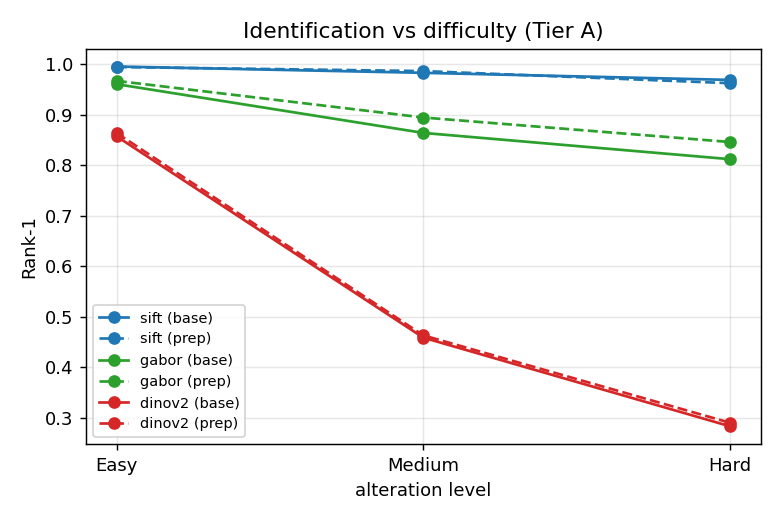
\includegraphics[width=0.72\textwidth]{figures/rank1_by_level.png}
\caption{Rank-1 in funzione della difficolt\`a. Linea continua = baseline,
tratteggiata = preprocessed.}
\label{fig:rank1}
\end{figure}

\subsection{Verifica: solo SIFT \`e usabile a soglia severa}

\begin{table}[h]
\centering
\begin{tabular}{@{}lcccccc@{}}
\toprule
& \multicolumn{2}{c}{\textbf{SIFT}} & \multicolumn{2}{c}{\textbf{Gabor}} & \multicolumn{2}{c}{\textbf{DINOv2}} \\
\cmidrule(lr){2-3}\cmidrule(lr){4-5}\cmidrule(lr){6-7}
(baseline) & EER & FAR@FRR1\% & EER & FAR@FRR1\% & EER & FAR@FRR1\% \\
\midrule
Easy   & 0.003 & 0.001 & 0.055 & 0.329 & 0.071 & 0.343 \\
Medium & 0.008 & 0.004 & 0.114 & 0.663 & 0.169 & 0.658 \\
Hard   & 0.010 & 0.011 & 0.131 & 0.773 & 0.198 & 0.755 \\
\bottomrule
\end{tabular}
\caption{Metriche di verifica (condizione baseline). SIFT ha EER e FAR@FRR=1\%
di ordini di grandezza inferiori.}
\label{tab:verif}
\end{table}

Al punto operativo severo (FAR@FRR=1\%, Tabella~\ref{tab:verif}) solo SIFT \`e
utilizzabile: il suo punteggio (numero di inlier) ha una separazione enorme tra
genuini e impostori. Gabor e DINOv2, pur avendo EER/AUC decenti, hanno code delle
distribuzioni fortemente sovrapposte e sono inservibili a FRR=1\% sulle
alterazioni difficili.

\subsection{Analisi per tipo di alterazione}

\begin{table}[h]
\centering
\begin{tabular}{@{}lccc@{}}
\toprule
Rank-1 a \emph{Hard} (baseline) & \textbf{SIFT} & \textbf{Gabor} & \textbf{DINOv2} \\
\midrule
CR (rotazione)      & 0.954 & 0.802 & 0.234 \\
Obl (obliterazione) & 0.964 & 0.654 & 0.310 \\
Zcut (taglio)       & 0.990 & 0.981 & 0.305 \\
\bottomrule
\end{tabular}
\caption{Rank-1 per tipo di alterazione al livello Hard.}
\label{tab:alt}
\end{table}

La Tabella~\ref{tab:alt} chiarisce i meccanismi. \textbf{DINOv2 fallisce su tutte}
le alterazioni difficili --- persino su un taglio pulito (Zcut, 0.305) che SIFT e
Gabor assorbono, perch\'e l'embedding globale non tollera una porzione mancante.
La \textbf{debolezza di Gabor \`e l'obliterazione} (0.654): la statistica di texture
degrada quando le creste sono distrutte, pur restando robusta al taglio (0.981).
\textbf{SIFT \`e robusto a tutte} (\(\geq0.954\)): la consistenza geometrica dei
keypoint sopravvive a rotazione, taglio e obliterazione parziale.

\subsection{L'effetto del preprocessing dipende dal modello}

\begin{table}[h]
\centering
\begin{tabular}{@{}lccc@{}}
\toprule
\(\Delta\)Rank-1 da preprocessing (punti \%) & Easy & Medium & Hard \\
\midrule
\textbf{Gabor}  & \(+0.7\) & \(+3.0\) & \(+3.4\) \\
\textbf{DINOv2} & \(+0.7\) & \(+0.5\) & \(+0.7\) \\
\textbf{SIFT}   & \(-0.1\)~(ns) & \(+0.4\)~(ns) & \(-0.6\)~(ns) \\
\bottomrule
\end{tabular}
\caption{Effetto del preprocessing sul Rank-1. Per SIFT il test appaiato (McNemar)
d\`a p-value non significativi a ogni livello (Easy 0.69, Medium 0.23, Hard 0.15);
i \(\Delta\)EER hanno intervalli di confidenza bootstrap che includono lo zero.}
\label{tab:prep}
\end{table}

Il risultato pi\`u sfumato (Tabella~\ref{tab:prep}, Figura~\ref{fig:prep}): la
maschera di contrasto \textbf{aiuta il descrittore di texture (Gabor), sempre di
pi\`u con la difficolt\`a}; \`e \textbf{marginale per l'embedding profondo} (DINOv2);
ed \`e \textbf{statisticamente neutra per il matcher di keypoint (SIFT)} --- pu\`o
addirittura peggiorarlo leggermente a Hard, poich\'e l'affilatura introduce keypoint
spuri e rompe la consistenza geometrica. Un preprocessing nato per la robustezza
facciale non \`e dunque un bene universale: il suo valore dipende dalla
rappresentazione a valle.

\begin{figure}[h]
\centering
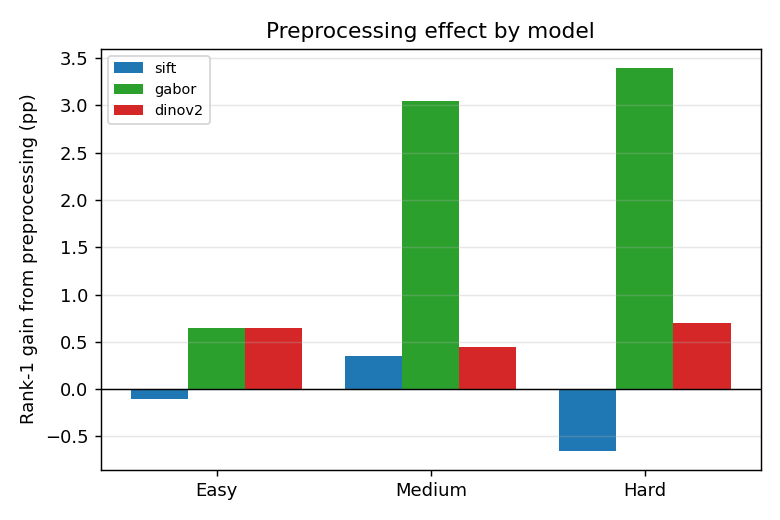
\includegraphics[width=0.66\textwidth]{figures/preprocessing_delta.png}
\caption{Guadagno di Rank-1 dal preprocessing, per modello e livello.}
\label{fig:prep}
\end{figure}

\section{Discussione e conclusioni}

Lo studio ribalta due volte l'intuizione comune. Primo: il modello profondo
pi\`u recente (DINOv2, \emph{frozen}) \`e il \textbf{peggiore} e collassa sulle
alterazioni difficili, mentre il metodo pi\`u classico (SIFT + RANSAC) \`e il
\textbf{migliore} e quasi non degrada. La ragione \`e strutturale: su impronte
alterate conta la robustezza \emph{locale e geometrica} (keypoint + RANSAC), non
la semantica globale di un embedding fuori distribuzione. Secondo: una pipeline di
preprocessing utile per un modello (Gabor) pu\`o essere neutra o dannosa per un
altro (SIFT), quindi il beneficio del preprocessing \`e \textbf{contingente alla
rappresentazione}, non universale.

\paragraph{Limitazioni.} SIFT \`e stato eseguito sul manifesto completo da
\num{2000} probe (come gli altri) solo dopo un compromesso iniziale a \num{500}
per il costo O(\(N\times\)galleria); il Tier B (set probe completo) resta
infattibile per SIFT. DINOv2 \`e usato esattamente come da specifica congelata
(CLS, 224 px), quindi il risultato riflette feature \emph{off-the-shelf} e non una
variante ad alta risoluzione o fine-tuned. La significativit\`a appaiata \`e
calcolata per SIFT; per Gabor/DINOv2 i \(\Delta\) sono stime puntuali (il
framework la calcola con \texttt{significance.py} sugli stessi \texttt{scores.jsonl}).

\paragraph{Riproducibilit\`a.} Tutta la casualit\`a (subsampling, campionamento
impostori, RANSAC) \`e seedata dal config; la cache della galleria \`e firmata dai
parametri; i risultati grezzi per-probe sono archiviati con snapshot della
configurazione e versioni delle librerie.

\end{document}
